\documentclass{beamer}
\usepackage{graphicx, parskip, microtype}
\usepackage{hyperref}

\frenchspacing

\usetheme{default}
\usecolortheme{whale}

\setbeamertemplate{navigation symbols}{}

\setbeamercolor{title}{fg=blue,bg=white}

\setbeamercolor{block title}{fg=white,bg=gray}
\setbeamercolor{block body}{fg=black,bg=lightgray}

\setbeamercolor{block title alerted}{fg=white,bg=darkgray}
\setbeamercolor{block body alerted}{fg=black,bg=lightgray}

\title{From the bottom of the wiki hole}
\author{Peter D Smits}
\institute{Committee on Evolutionary Biology, University of Chicago}

\begin{document}

\begin{frame}
  \maketitle
\end{frame}

\begin{frame}
  \frametitle{or\dots}
  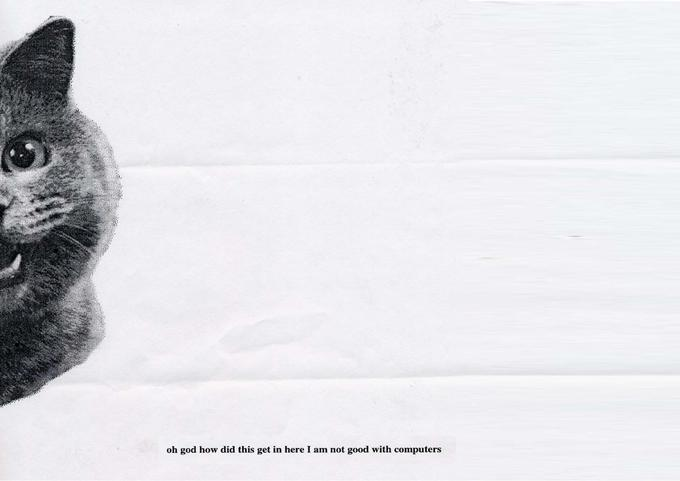
\includegraphics[width = \textwidth, keepaspectratio = true]{figure/happy_cat}
\end{frame}

\begin{frame}
  \frametitle{What?}
  \begin{center}
    
\includegraphics[height = 0.8\textheight, keepaspectratio = true]{figure/wiki}
  \end{center}
\end{frame}

\begin{frame}
  \frametitle{How many?}
  \begin{center}
    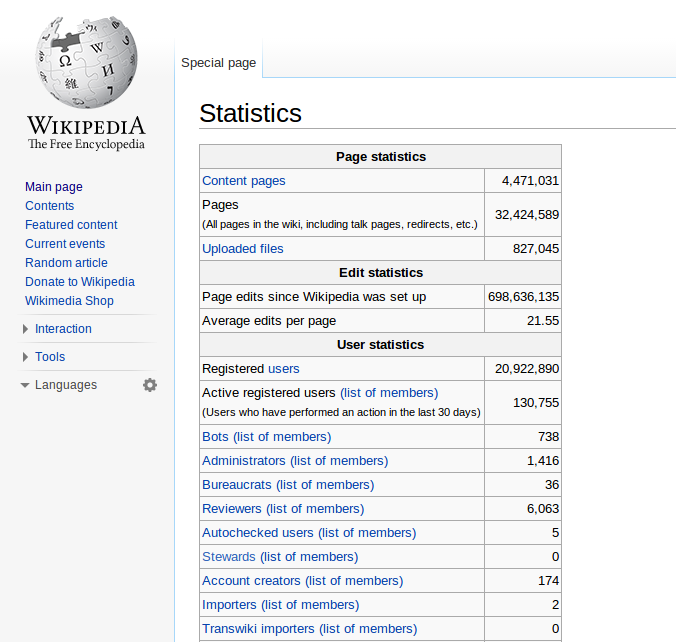
\includegraphics[height = 0.8\textheight, keepaspectratio = true]{figure/wiki_stats}
  \end{center}
\end{frame}

\begin{frame}
  \frametitle{Just how much time could I waste?}

  Read rate: 600 wpm, 16 hours/day = 17,000,000 words/month. 
  
  It would take \textbf{7} (!!!!!!) years to read wikipedia if it remained static. 
\end{frame}

\begin{frame}
  \frametitle{at about 1:19 this afternoon\ldots}
  \begin{center}
    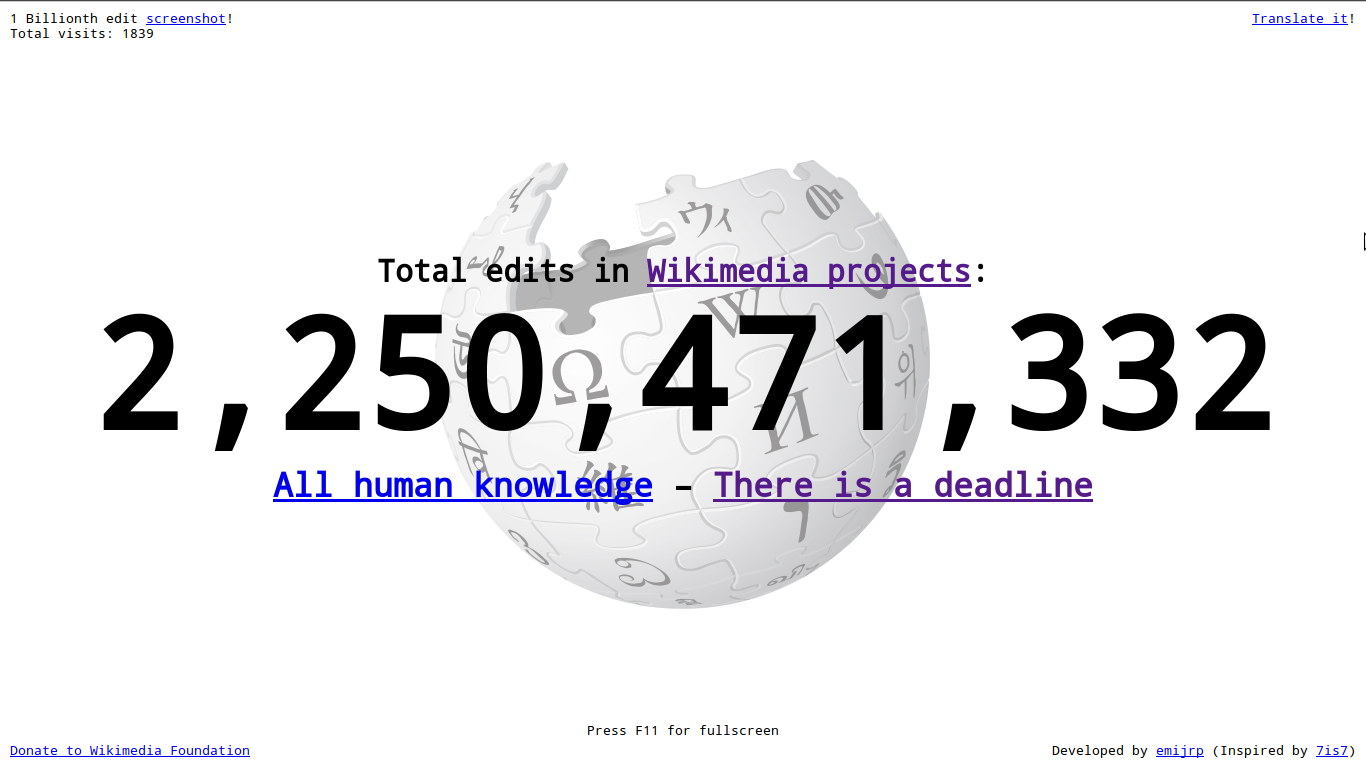
\includegraphics[height = 0.8\textheight, width = \textwidth, keepaspectratio = true]{figure/edits}
  \end{center}
\end{frame}

\begin{frame}
  \frametitle{Who?}
  \begin{center}
    
\includegraphics[height = 0.8\textheight, keepaspectratio = true]{figure/wiki_family}
  \end{center}
\end{frame}

\begin{frame}
  \frametitle{Go ahead and take my money}
  \begin{center}
    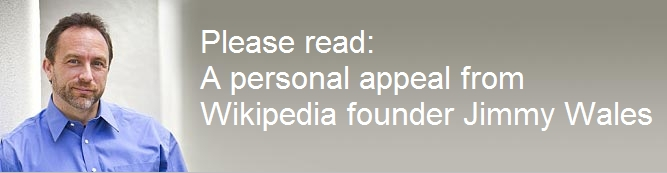
\includegraphics[width = \textwidth, height = 0.2\textheight, keepaspectratio = true]{figure/appeal_1}

    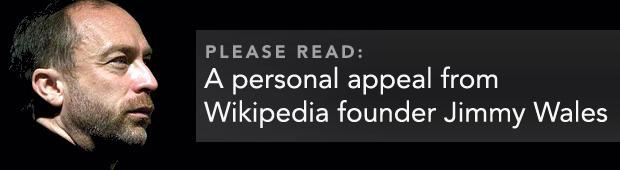
\includegraphics[width = \textwidth, height = 0.2\textheight, keepaspectratio = true]{figure/appeal_2}

    
\includegraphics[width = \textwidth, height = 0.2\textheight, keepaspectratio = true]{figure/appeal_3}

    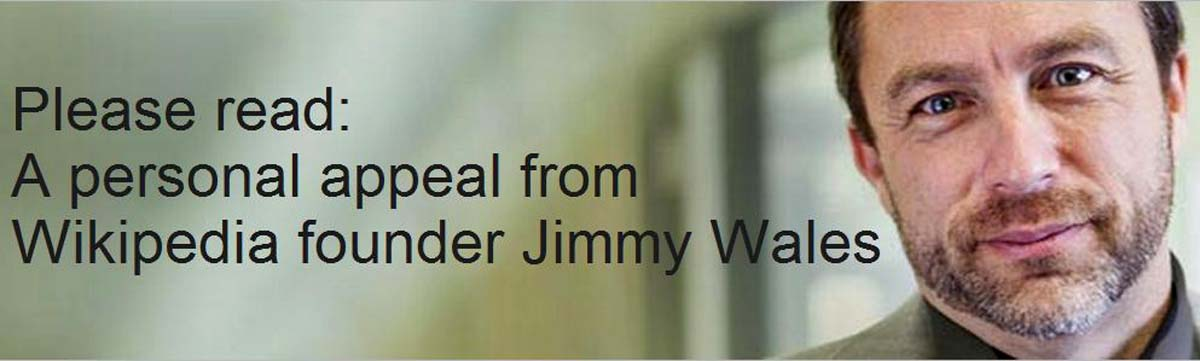
\includegraphics[width = \textwidth, height = 0.2\textheight, keepaspectratio = true]{figure/appeal_4}
  \end{center}
\end{frame}

\begin{frame}
  \frametitle{Problems? In my wiki?}
  \begin{center}
    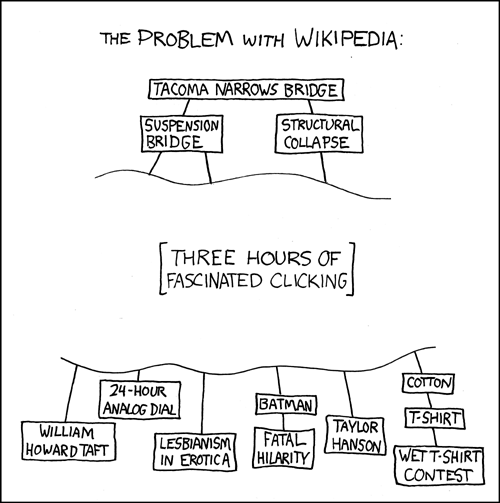
\includegraphics[height = 0.8\textheight, keepaspectratio = true]{figure/the_problem_with_wikipedia}
  \end{center}
\end{frame}

\begin{frame}
  \frametitle{Thar be dragons}

  \url{http://en.wikipedia.org/wiki/Special:Random}
\end{frame}

\begin{frame}
  \frametitle{Oh no pigeons}
  \begin{center}
    
\includegraphics[width = \textwidth, keepaspectratio = true]{figure/wiki_game}
  \end{center}
\end{frame}

\begin{frame}
  \frametitle{There is more than one wiki?}
  \begin{center}
    
\includegraphics[width = \textwidth, keepaspectratio = true]{figure/wikia}
  \end{center}
\end{frame}

\begin{frame}
  \frametitle{wiki-ing intensifies}
  \begin{center}
    \noindent
    
\includegraphics[width = 0.3\textwidth, keepaspectratio = true]{figure/tropes}\hspace{0.2\textwidth}
    
\includegraphics[width = 0.4\textwidth, height = 0.4\textheight, keepaspectratio = true]{figure/memalpha1}\\[2em]
    
\includegraphics[width = 0.4\textwidth, height = 0.4\textheight, keepaspectratio = true]{figure/wookie}\hspace{0.2\textwidth}
    
\includegraphics[width = 0.4\textwidth, height = 0.4\textheight, keepaspectratio = true]{figure/bulbapedia}\par
  \end{center}
\end{frame}

\begin{frame}
  \frametitle{heavy breathing}
  \begin{center}
    
\includegraphics[width = \textwidth, keepaspectratio = true]{figure/ice}

    
\includegraphics[width = 0.6\textwidth, keepaspectratio = true]{figure/got}
  \end{center}
\end{frame}

\begin{frame}
  \frametitle{nothing is sacred}
  \begin{columns}
    \begin{column}{0.5\textwidth}
      
\includegraphics[width = \textwidth, height = 0.4\textheight, keepaspectratio = true]{figure/seinfeld}

      \vspace{2cm}

      
\includegraphics[width = \textwidth, height = 0.4\textheight, keepaspectratio = true]{figure/dragonball}
    \end{column}
    \begin{column}{0.5\textwidth}
      
\includegraphics[width = \textwidth, height = 0.4\textheight, keepaspectratio = true]{figure/simpsons_1}

      \vspace{1cm}

      
\includegraphics[width = \textwidth, height = 0.4\textheight, keepaspectratio = true]{figure/simpsons_2}
    \end{column}
  \end{columns}
\end{frame}

\begin{frame}
  \frametitle{scariest link on the internet}

  \url{http://tvtropes.org/pmwiki/randomitem.php?p=1}

  you might loose 1 to 24 hours if you go to this link. and possibly your sanity.
\end{frame}

\begin{frame}
  \frametitle{let the wookie win}
  \begin{columns}
    \begin{column}{0.5\textwidth}
      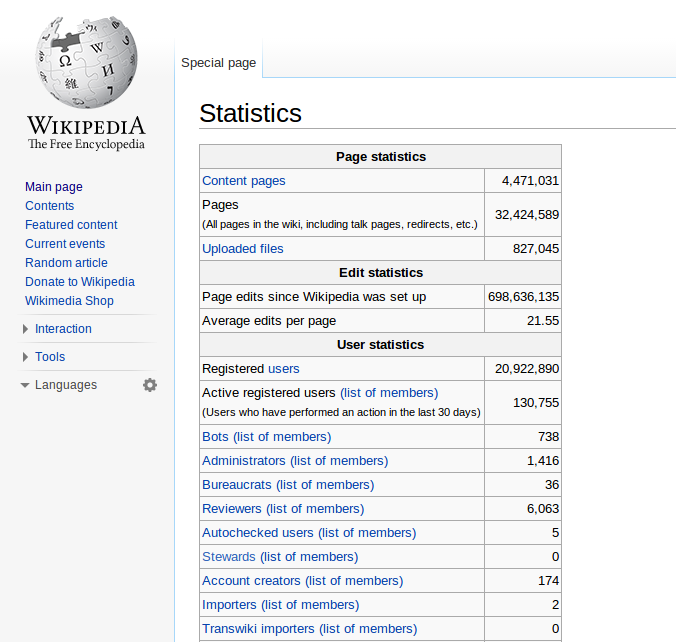
\includegraphics[height = 0.8\textheight, width = \textwidth, keepaspectratio = true]{figure/wiki_stats}
    \end{column}
    \begin{column}{0.5\textwidth}
      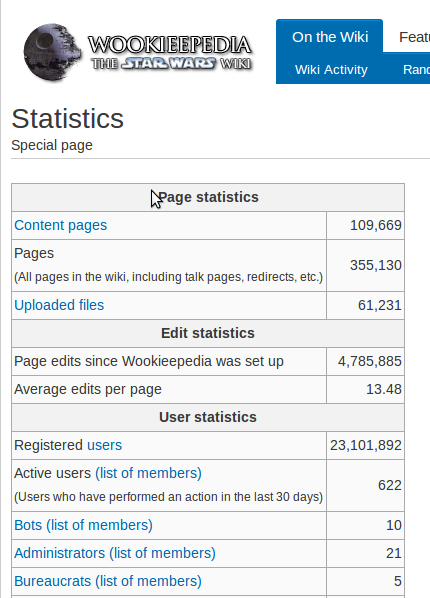
\includegraphics[height = 0.8\textheight, width = \textwidth, keepaspectratio = true]{figure/wookie_stats}
    \end{column}
  \end{columns}
\end{frame}

\begin{frame}
  \frametitle{gotta catch 'em all}
  \begin{columns}
    \begin{column}{0.5\textwidth}
      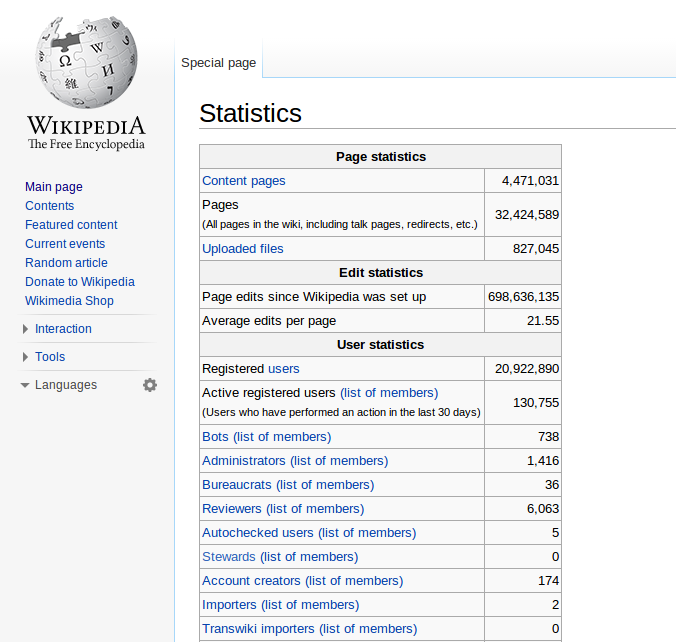
\includegraphics[height = 0.8\textheight, width = \textwidth, keepaspectratio = true]{figure/wiki_stats}
    \end{column}
    \begin{column}{0.5\textwidth}
      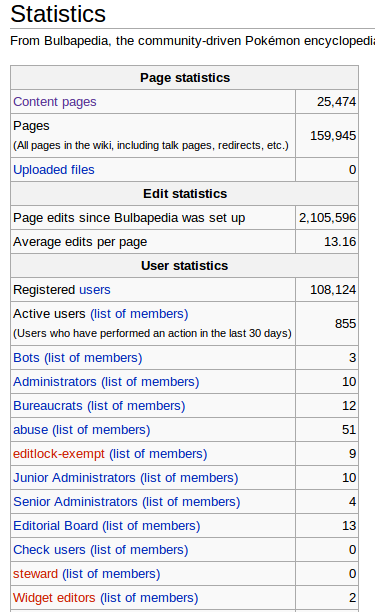
\includegraphics[height = 0.8\textheight, width = \textwidth, keepaspectratio = true]{figure/bulb_stats}
    \end{column}
  \end{columns}
\end{frame}

\begin{frame}
  \frametitle{facepalm}
  \begin{columns}
    \begin{column}{0.5\textwidth}
      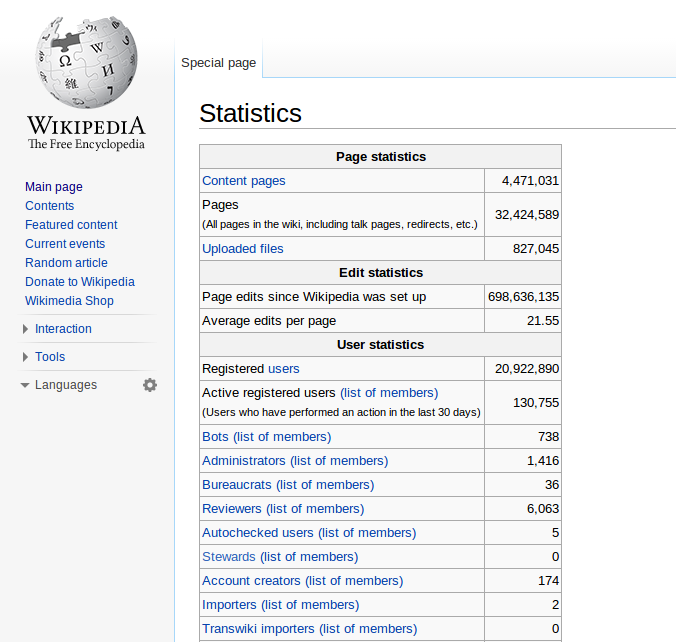
\includegraphics[height = 0.8\textheight, width = \textwidth, keepaspectratio = true]{figure/wiki_stats}
    \end{column}
    \begin{column}{0.5\textwidth}
      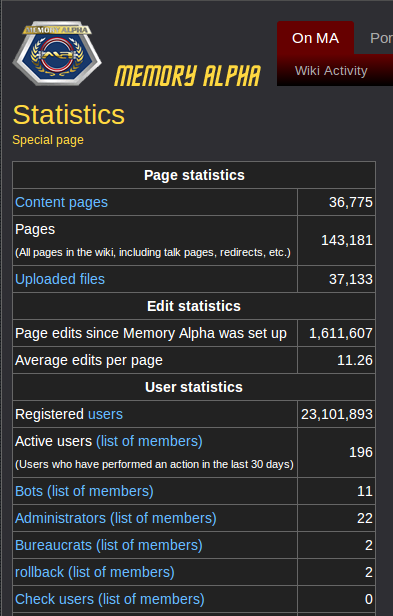
\includegraphics[height = 0.8\textheight, width = \textwidth, keepaspectratio = true]{figure/trek_stats}
    \end{column}
  \end{columns}
\end{frame}

\begin{frame}
  \frametitle{Analysis time!}
  \begin{center}
    
\includegraphics[height = 0.8\textheight, width = \textwidth, keepaspectratio = true]{figure/star-trek-insignia}
  \end{center}
\end{frame}

\begin{frame}
  \frametitle{tl;dr}
  \begin{itemize}
    \item memory alpha dump
      \begin{itemize}
        \item XML format
        \item every, and i mean every, current page
        \item no images
        \item \~{} 313 MB
      \end{itemize}
    \item R plus packages
      \begin{itemize}
        \item see what you can do with your degree?
      \end{itemize}
    \item link network. content pages. both in and out of universe.
      \begin{itemize}
        \item cut out admin pages (help, users, etc.)
        \item my cleaning might have confused the characters from TOS with those from the newest films. whatever. this is informal and i can always fix it later. 
      \end{itemize}
  \end{itemize}
\end{frame}

\begin{frame}
  \frametitle{Questions}
  \huge{Captains? (and commander\ldots )}

  \huge{Series?}

  \huge{etc.}
\end{frame}

\begin{frame}
  \frametitle{summaries}

  nodes: 34366

  links: 788851

  diameter: 10

  mean links: \~{} 45; median: 19

  closeness centrality: \(8.72 \cdot 10^{-6}\)
\end{frame}

\begin{frame}
  \frametitle{emergent structure?}
  yeah\ldots but graph is still too huge to show. sorry.

  1040 modules (173 modules of size 1)

  56358 links
\end{frame}

\begin{frame}
  \frametitle{module sizes}
  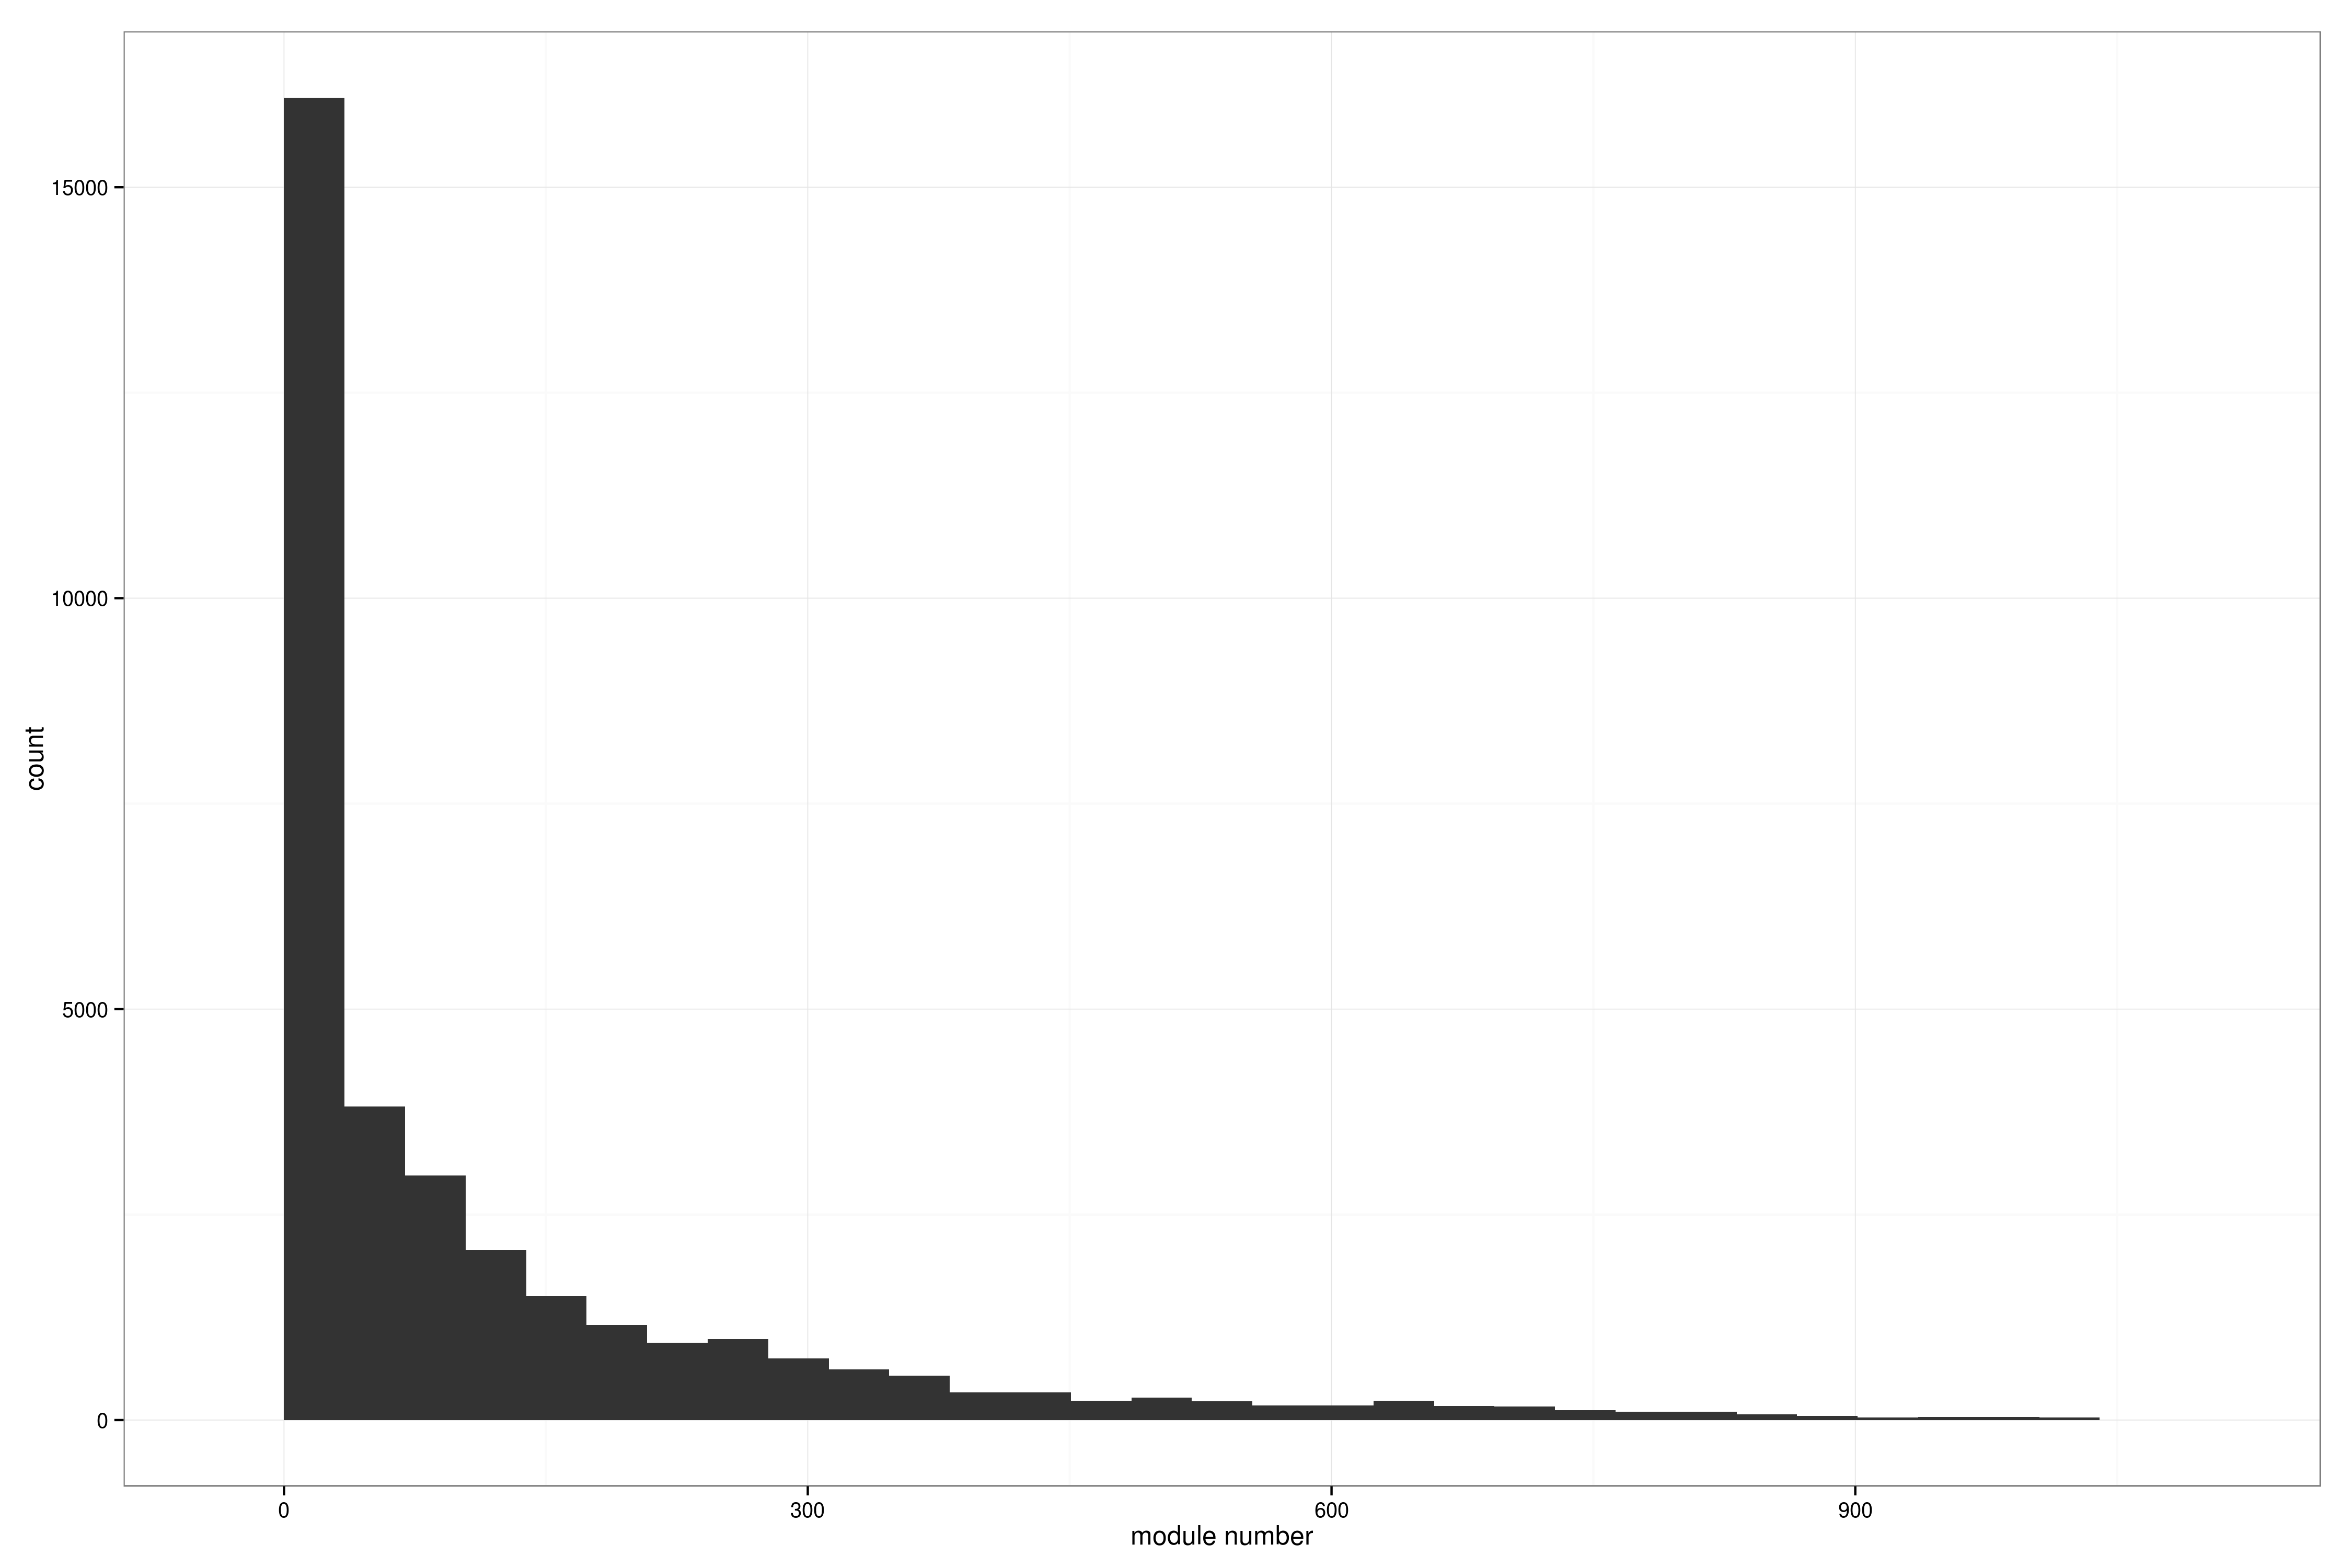
\includegraphics[height = 0.8\textheight, keepaspectratio = true]{figure/modules}
\end{frame}

\begin{frame}
  \frametitle{module degree}
  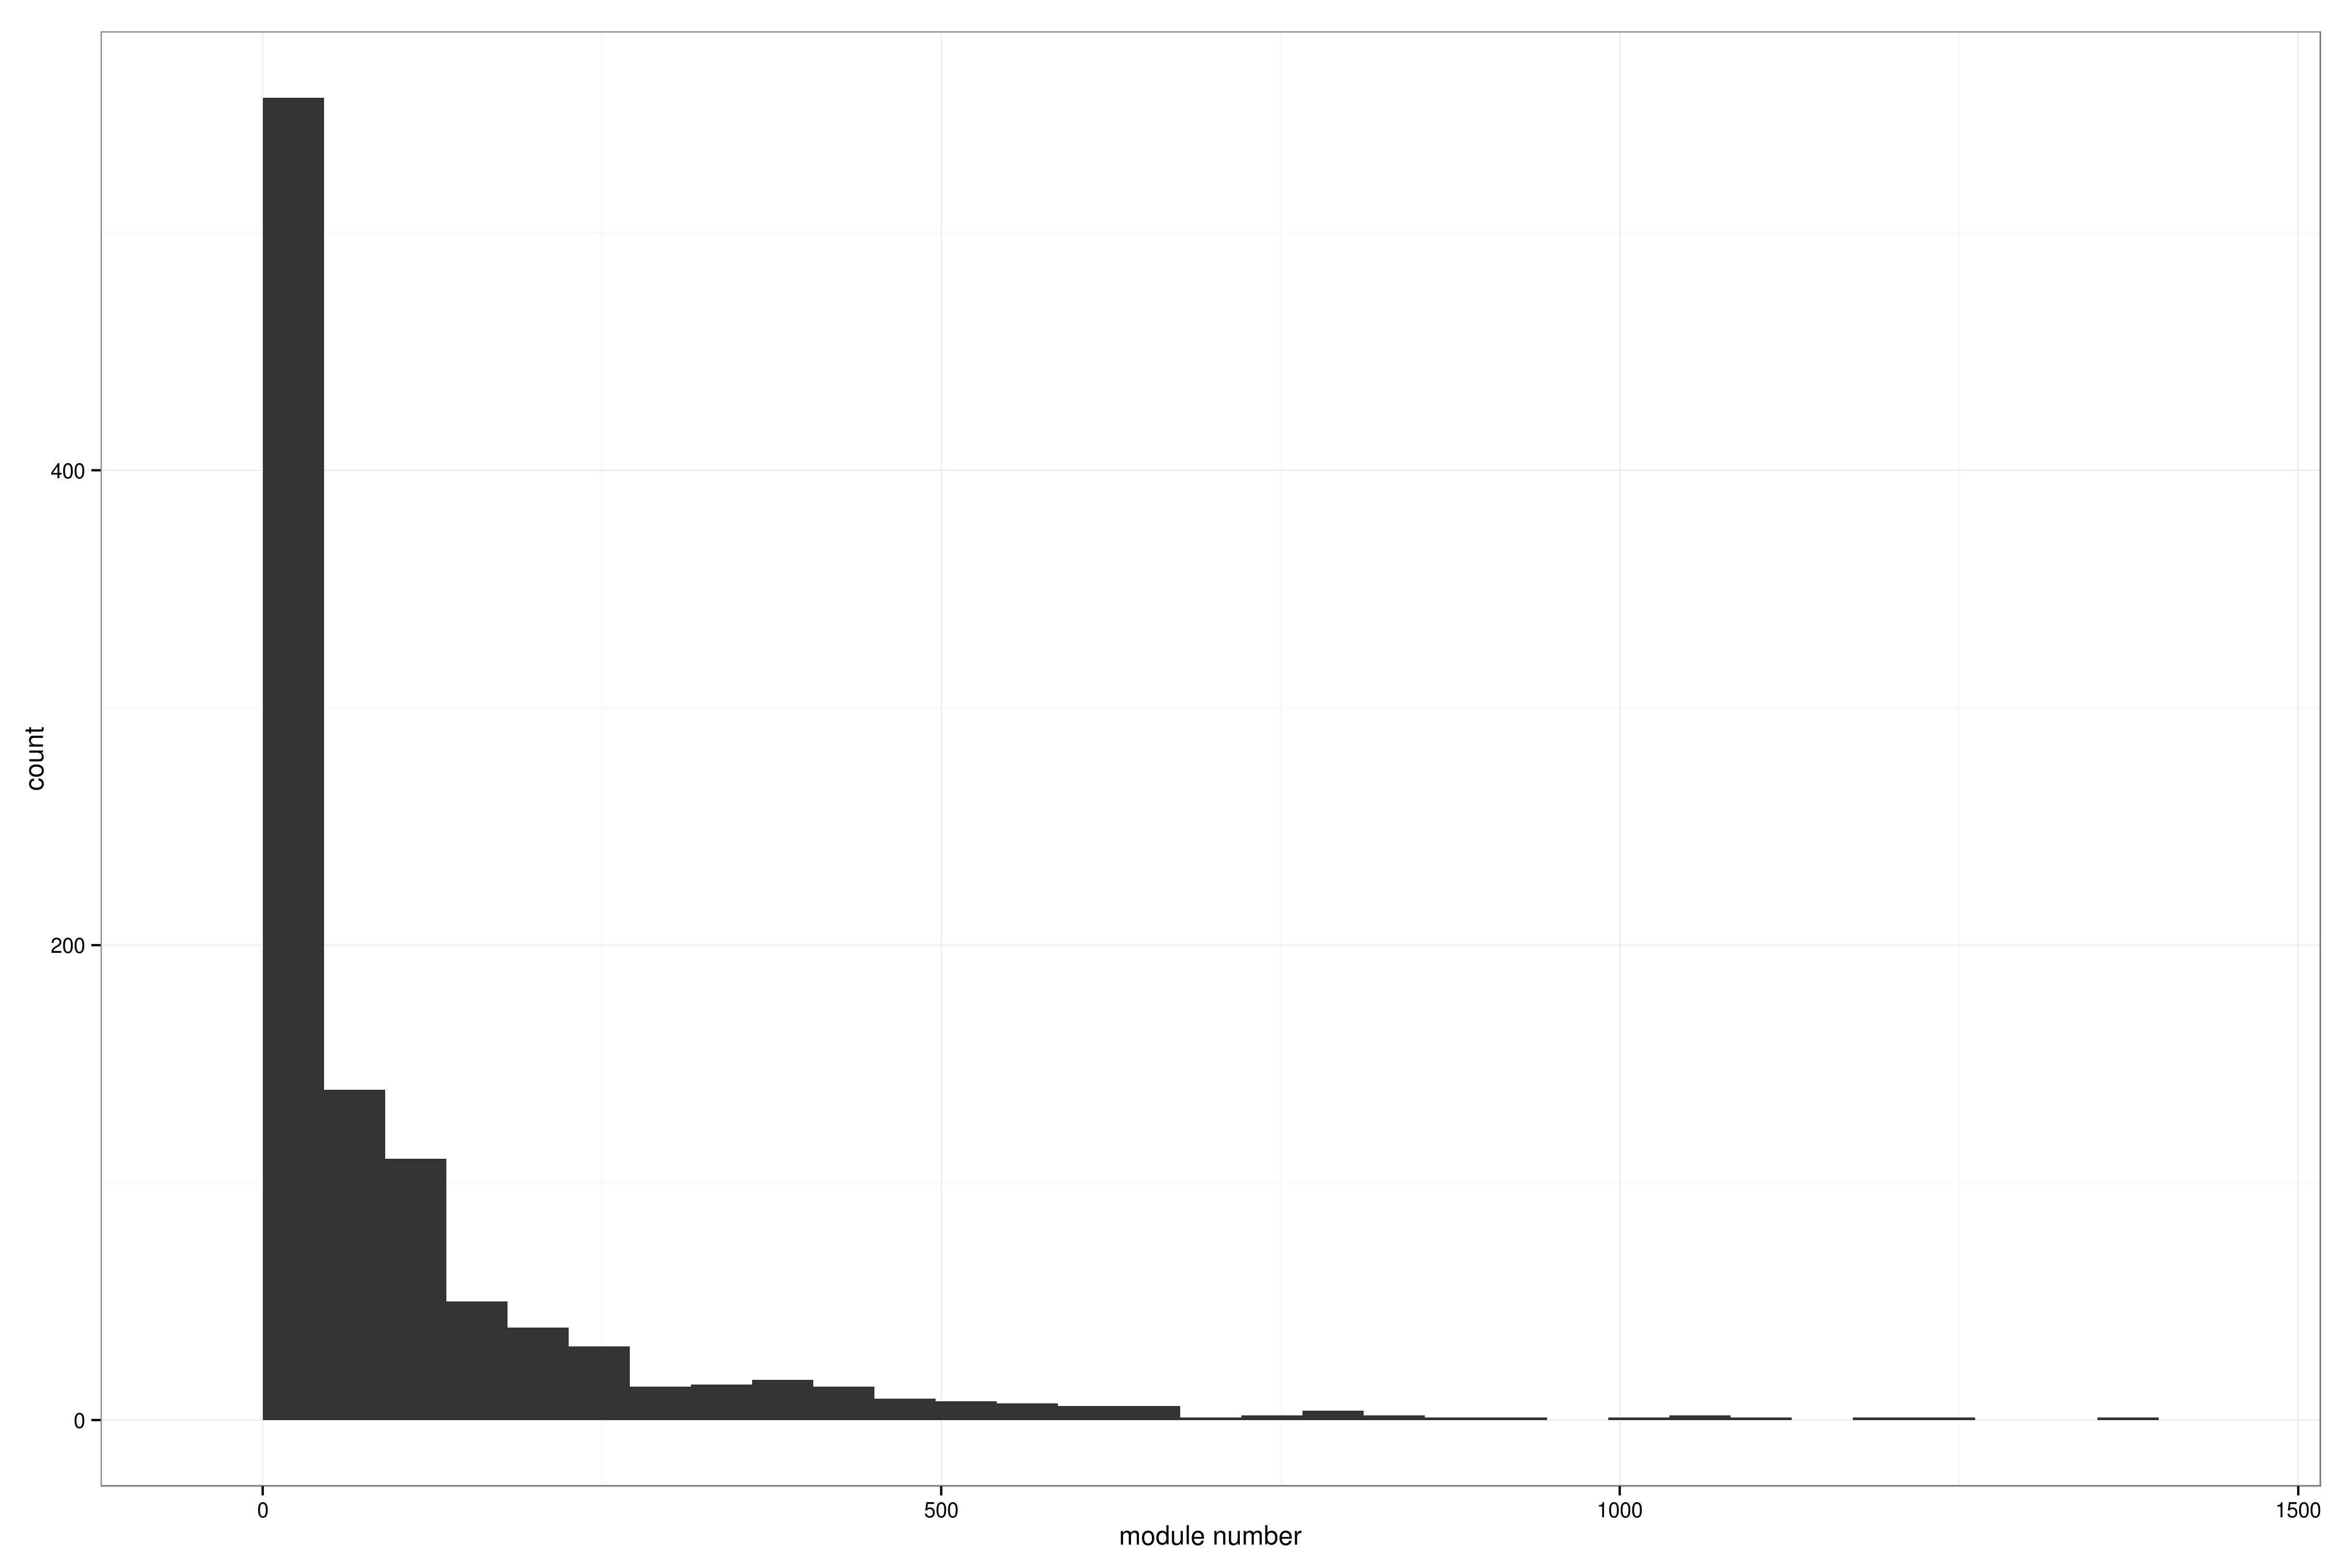
\includegraphics[height = 0.8\textheight, keepaspectratio = true]{figure/mod_deg}
\end{frame}

\begin{frame}
  \frametitle{We have them just where they want us}
  What's in the first box? First few important things\ldots

  \begin{itemize}
    \item william shatner
    \item j. j. abrams
    \item leonard nimoy
    \item jonathan frakes
    \item patrick stewart
    \item roberto orci (wrote recent star trek film)
    \item robert picardo (the doctor from voyager)
  \end{itemize}

  real people. boring.
\end{frame}

\begin{frame}
  \frametitle{Other boxes?}
    \begin{itemize}
      \item 2: deep space 9 and related things
      \item 3: TOS and related things
      \item 4: enterprise (series) and related
      \item 5: planets and space
      \item 6: star fleet
      \item 7: voyager, borg, and related
      \item 8: klingons
      \item 9: production staff and related
    \end{itemize}

    smaller boxes overlap a little, but there is a ``structure''
\end{frame}

\begin{frame}
  \frametitle{10 most important pages/``things''}
  \begin{enumerate}
    \item<10-> captain
    \item<9-> earth
    \item<8-> starfleet
    \item<7-> federation
    \item<6-> planet
    \item<5-> star trek (out of universe)
    \item<4-> star trek: the next generation
    \item<3-> starship
    \item<2-> human
    \item<1-> star trek: deep space nine
  \end{enumerate}
\end{frame}

\begin{frame}
  \frametitle{weirdest click series}

  tanagra family

  gallos ii

  inhabited planets

  23rd century

  san francisco

  san francisco herald

  jessica bradley

  encounter at farpoint

  henry vi, part iii

  the naked now

  decontamination

\end{frame}

\begin{frame}
  \frametitle{series}
  \begin{columns}
    \begin{column}{0.5\textwidth}
      
\includegraphics[width = \textwidth, keepaspectratio = true]{figure/tos}

      \vspace{1cm}

      
\includegraphics[width = \textwidth, keepaspectratio = true]{figure/ds9}
    \end{column}
    \begin{column}{0.5\textwidth}
      
\includegraphics[width = \textwidth, keepaspectratio = true]{figure/tng}

      \vspace{0.5cm}

      
\includegraphics[width = \textwidth, keepaspectratio = true]{figure/voy}
    \end{column}
  \end{columns}
\end{frame}

\begin{frame}
  \frametitle{series}
  % latex table generated in R 3.0.2 by xtable 1.7-1 package
% Fri Mar 14 11:21:19 2014
\begin{table}[ht]
\centering
\begin{tabular}{rrrr}
  \hline
 & page.rank & degree & closeness \\ 
  \hline
star trek: the next generation & 0.0049 & 2658 & 0.00039 \\ 
  star trek: deep space nine & 0.0041 & 4286 & 0.00039 \\ 
  star trek: voyager & 0.0034 & 2261 & 0.00039 \\ 
  star trek: enterprise & 0.0030 & 1929 & 0.00039 \\ 
  star trek: the original series & 0.0028 & 3367 & 0.00039 \\ 
   \hline
\end{tabular}
\end{table}

\end{frame}

\begin{frame}
  \frametitle{captains}
  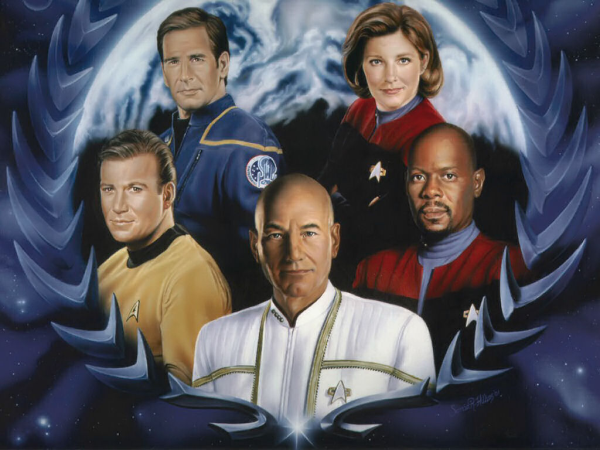
\includegraphics[height = 0.8\textheight, keepaspectratio = true]{figure/Star-Trek-Captains}
\end{frame}

\begin{frame}
  \frametitle{captains}
  % latex table generated in R 3.0.2 by xtable 1.7-1 package
% Fri Mar 14 11:22:42 2014
\begin{table}[ht]
\centering
\begin{tabular}{rrrr}
  \hline
 & page.rank & degree & closeness \\ 
  \hline
jean-luc picard & 0.00334 & 3808 & 0.00039 \\ 
  james t. kirk & 0.00329 & 2380 & 0.00039 \\ 
  benjamin sisko & 0.00238 & 1925 & 0.00039 \\ 
  kathryn janeway & 0.00207 & 3586 & 0.00039 \\ 
  jonathan archer & 0.00167 & 2311 & 0.00039 \\ 
   \hline
\end{tabular}
\end{table}

\end{frame}

\begin{frame}
  \frametitle{obviously}
  
\includegraphics[width = \textwidth, keepaspectratio = true]{figure/win}
\end{frame}


\end{document}
